\documentclass{beamer}
%
% Choose how your presentation looks.
%
% For more themes, color themes and font themes, see:
% http://deic.uab.es/~iblanes/beamer_gallery/index_by_theme.html
%
\mode<presentation>
{
  \usetheme{default}      % or try Darmstadt, Madrid, Warsaw, ...
  \usecolortheme{beaver} % or try albatross, beaver, crane, ...
  \usefonttheme{default}  % or try serif, structurebold, ...
  \setbeamertemplate{navigation symbols}{}
  \setbeamertemplate{caption}[numbered]
}

\usepackage[english]{babel}
\usepackage[utf8x]{inputenc}
\usepackage{mathtools}
\usepackage{blkarray}

\title[Ron Graham's Sequence]{Ron Graham's Sequence}
\subtitle{and the On-Line Encylopedia of Integer Sequences}
\author{Peter Kagey}
\institute{University of Southern California}
\date[]{
  Graduate Student Combinatorics Conference\\
  April 8, 2018
}

\begin{document}

\begin{frame}
  \titlepage
\end{frame}

% Uncomment these lines for an automatically generated outline.
%\begin{frame}{Outline}
%  \tableofcontents
%\end{frame}

% \section{Introduction}
%
% \begin{frame}{Introduction}
%
%   \begin{block}{About me}
%   \begin{itemize}
%   \item B.S. in Math from Oregon State University in 2014.
%   % This means that I have less credentials/experience than most of the folks who speak at this lecture
%   % I switched to study math at the end of my Junior year, and took math classes full time to finish with
%   % A B.S. in Math in three terms. During my second term, I took MTH 342 for a graduation requirement, but
%   % This was after having taken MTH 256 (a half term of linear algebra), MTH 341 (a class that I
%   % didn't regularly attend where the lectures seemed to be principally about pivot columns and
%   % Gaussian elimination, and MTH 451 (Numerical Linear Algebra). So by the time Linear Algebra II came
%   % around, I had already covered about 80% of the material in other classes. However, it turned out that
%   % because I had some experience with doing elementary linear algebra, I had the mental constructs I
%   % needed to make good sense of the material that I didn't know, and so I finished that course with
%   % feelings of mastery, and I think it may have been one of my best course experiences at OSU.
%   % With all that said, I have a suspicion that your experience with this talk may be like my experience
%   % with basic linear algebra—you likely know more than I do about many of the topics that I'll be chatting
%   % about, but hopefully that means that you can get a deep understanding about the problem I'll be talking
%   % about, and event more hopefully that means you can ask some insightful questions
%   % (that I may or may not know the answers to!) So I hope that this talk will be interesting despite being
%   % perhaps the most elementary lecture given at this seminar.
%   % At the very least, hopefully I can inspire you with my childlike wonder.
%   \item Wrote back-end web software for a medical device company in Portland from 2014-2017.
%   % Note: I spent the first number of months reverse-engineering the byte-code of blood glucose monitor
%     protocols, so I'm weirdly comfortable looking at 1s and 0s.
%   \item Authored 180+ sequences in the OEIS (On-Line Encyclopedia of Integer Sequences).
%   % Let's show off OEIS for a few minutes?
%   %   275k+ sequences.
%   %   Prime numbers
%   %   Fibonacci sequence
%   %   Tribonacci sequence
%   \end{itemize}
%   \end{block}
%
% \end{frame}

% \begin{frame}{About Ron Graham's sequence}
%   \begin{itemize}
%   \item A bijection from the natural numbers to the (positive) non-prime integers.
%   \item A variant of the sequence appeared as problem A2 on the 2013 Putnam Exam.
%   \item The earliest published reference to this sequence is from September 1988
%       in the first edition of \textit{Concrete Mathematics: A Foundation for Computer Science}
%       by Ron Graham, Donald E. Knuth, and Oren Patashnik.
%   \item First appears in the OEIS in 1991 with 25 known terms
%   \item Extended to 54 terms in 1994, 70 terms in 2003, and 125 terms in 2014.
%   \item At the end of 2014, I discovered an algorithm that extended the sequence to 10,000
%         terms and uncover six errors between the 84th and 104th terms.
%   \end{itemize}
% \end{frame}

\begin{frame}{Genesis}
  \begin{block}{Putnam 2013 A2}
    Consider choices of integers $b_1,b_2,\dots, b_t$ such that
    $n<b_1<b_2<\cdots<b_t$ and $n\cdot b_1\cdot b_2\cdots b_t$ is a perfect square,
    and let $g(n)$ be the minimum of $b_t$ over all such choices.
    \\ ~ \\
    For example, $2\cdot 3\cdot 6$ is a perfect square, while
    $2\cdot 3,2\cdot 4, 2\cdot 5, 2\cdot 3\cdot 4,$ $2\cdot 3\cdot 5, 2\cdot 4\cdot 5,$
    and $2\cdot 3\cdot 4\cdot 5$ are not, and so $g(2)=6.$
    \\ ~ \\
    Show that the function $g$ from $\mathbb{N}$ to\
     $\mathbb{N}$ is
    one-to-one.
  \end{block}
\end{frame}

% https://oeis.org/A285521
% https://oeis.org/A298121
% https://oeis.org/A300002
% https://oeis.org/A278299
% https://oeis.org/A300444
\begin{frame}{The On-Line Encylopedia of Integer Sequences}
  \begin{itemize}
    \item The On-Line Encylopedia of Integer Sequences was started by
      Neil Sloane in 1964 as a graduate student at Cornell.
    \item In 1996, the database made its way to the internet.
    \item The OEIS contains over 300000 sequences.
    \item It is a good resource for finding references, generating functions,
      recurrences, plots, etc. about integer sequences.
    \item Roughly 100 new sequences are added every day after being reviewed by
      a team of volunteer editors.
    % 2010 AMS/MAA meeting.
    \center{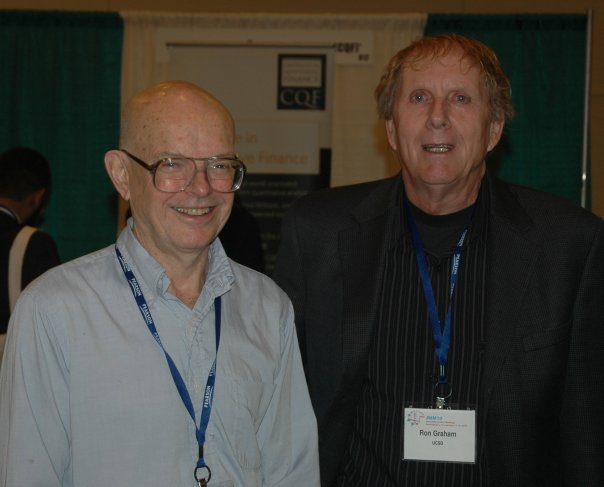
\includegraphics[scale=0.3,trim={0 5cm 0 1cm},clip]{Ron_Graham_Neil_Sloane.jpg}}
  \end{itemize}
\end{frame}

\begin{frame}{Definition (OEIS A006255)}
  % g(n) is defined by the least upper bound of a strictly increasing sequence starting at n
  % with the property that the product of the sequence is a square.
  Let $g(n)$ be the smallest $m$ for which there exists a strictly increasing \textbf{square sequence}:
    \[n = b_1 < b_2 < \cdots < b_t = m\]
  where
    \[b_1 \cdot b_2 \hdots b_t \text{ is square}\]

  \begin{block}{Examples}
    \setlength\abovedisplayskip{-10pt}
    \begin{alignat*}{3}
      & g(2) = 6  && \qquad\quad 2 \cdot 3 \cdot 6  &&= 6^2  \\
      & g(3) = 8  && \qquad\quad 3 \cdot 6 \cdot 8  &&= 12^2 \\
      & g(4) = 4  && \qquad\quad 4                  &&= 2^2  \\
      & g(5) = 10 && \qquad\quad 5 \cdot 8 \cdot 10 &&= 20^2 \\
      & \cdots    &&                                &&       \\
      & g(14) = 21 && \qquad\quad 14 \cdot 15 \cdot 18 \cdot 20 \cdot 21 &&= 1260^2
    \end{alignat*}
  \end{block}
\end{frame}

\begin{frame}{Naïve, brute-force algorithm}
  \begin{block}{Example: Computing $g(3)$}
    All strictly increasing sequences of numbers starting with $3$
    until a square sequence is reached:
    % These are sorted by lexicographic order of the sequence backward.
    \begin{alignat*}{2}
      \sqrt{3}             	   &= \sqrt{3}\\
      \sqrt{3 \cdot 4}         &= 2\sqrt{3}\\
      \sqrt{3 \cdot 5}         &= \sqrt{15}\\
      \sqrt{3 \cdot 4 \cdot 5} &= 2\sqrt{15}\\
      \sqrt{3 \cdot 6}         &= 3\sqrt{2}\\
      \cdots \\
      \sqrt{3 \cdot 6 \cdot 8} &= 12
    \end{alignat*}

    There are heuristics can be used to filter out many sequences, but in
    general this procedure takes exponential time.
  \end{block}
\end{frame}

\begin{frame}{Background}
  \begin{itemize}
    \item This problem first appeared as problem proposed by Ron Graham
          in the June 1987 edition of \textit{MAA Mathematics Magazine}.
    \item The problem later appears in September 1988 in the first edition of
      \textit{Concrete Mathematics} in by Ron Graham, Don Knuth, and Oren Patashnik.
    \item Appears in the OEIS in 1991 with 25 known terms.
    \item Extended to 54 terms in 1994, 70 terms in 2003, and 125 terms in 2014.
    \item At the end of 2014, the sequence was extended to 10,000 terms
          and six errors between the 84th and 104th terms were corrected.
  \end{itemize}
\end{frame}

\begin{frame}{Info}
  \begin{itemize}
    \item $g(n) \leq 4n$ because $n \cdot 4n = (2n)^2$
    \item $g(n) \leq 2n$ for $n \geq 4$
      \begin{itemize}
        \item For $n \geq 10$ there exists $k$ with $n < 2k^2 < 2n$.
      \end{itemize}
    \item In particular, $g(p) = 2p$ for any prime $p > 3$.
    \item $g(n)$ is a bijection from the natural numbers to the non-prime numbers.
    \item For any fixed integer $k$, $g(k\cdot p) = (k + 1)\cdot p$ if $p$ is a
      sufficiently large prime.
  \end{itemize}
\end{frame}

% Usually this upper bound is usually worse, but it has interesting properties
% of its own.
% \begin{frame}{Another upper bound}
%   \begin{block}{Definition}
%   Let $\bar{g}(n): \mathbb{N} \to \mathbb{N}$
%   be defined as the least $k > n$ such that $nk$ is a perfect square. \\
%   \end{block}
%
%   \begin{block}{Examples}
%   \setlength\abovedisplayskip{-10pt}
%   \begin{alignat*}{3}
%     & \bar{g}(2)  = 8  &&\text{ because } 2  \cdot 8  &&= 4^2\\
%     & \bar{g}(4)  = 9  &&\text{ because } 4  \cdot 9  &&= 6^2\\
%     & \bar{g}(50) = 72 &&\text{ because } 50 \cdot 72 &&= 60^2
%   \end{alignat*}
%   \end{block}
%   \begin{block}{Exercise}
%     Prove that $\bar{g}$ is 1-1 and onto the nonsquarefree numbers.
%   \end{block}
%   \begin{block}{Note}
%     % "Length-2 sequence"
%     It is an open problem whether or not there exists some $n$ such that $\bar{g}(n) = g(n)$.
%   \end{block}
% \end{frame}

\begin{frame}{2013 Putnam A2: $g$ is one-to-one.}
  \begin{proof}
    Assume that $m < n \leq g(m) = g(n)$ and denote the product sequences as:
    %        Without loss of generality, let $a < b < f(a) = f(b)$. \\
    %        The product of two squares is square: $(a \cdot f(a)) \cdot (b \cdot f(b))$ \\
    %        Thus $a \cdot b \cdot f(a)^2$ and $a \cdot b$ are square---a contradiction. \\
    %        This implies that f is 1-to-1.
    \begin{alignat*}{4}
      A &= \{n &= a_1 , a_2 , &\cdots &, a_t = g(n) &\} \\
      B &= \{m &= b_1 , b_2 , &\cdots &, b_s = g(m) &\}
    \end{alignat*}
    % 12 \cdot 18          \cdot 24 =  72^2
    % 15 \cdot 18 \cdot 20 \cdot 24 = 360^2
    Then the symmetric difference $A \triangle B$ defines a sequence which
    contradicts the hypothesis: \begin{enumerate}
      \item $\min(A \triangle B) = m$.
      \item $\max(A \triangle B) < g(m)$.
      \item $\operatorname{prod}(A \triangle B)$ is square.
    \end{enumerate}
  \end{proof}
\end{frame}

% \begin{frame}{Surjection}
%   \begin{block}{Claim}
%       The image of $g$ is the non-prime numbers.
%     \end{block}
%
%   \begin{proof}
%       Let $m$ be a positive, non-prime integer.\\
%         There exists a strictly increasing square sequence ending with $m$. \\
%         %(The prime factorization of the squarefree part of $y$. (e.g. $54 = 2*3^3$, so the sequence $2 \cdot 3 \cdot 54$ has a square product.)
%         Consider all such sequences, and take the one that maximizes the first term, call this term $n$.
%         This implies that $g(n) <= m$.\\
%         In particular, $g(n) = m$. If you assume that $g(n) < m$, and let\\
%           $A = \{n = a_1, a_2, ..., a_k = m\}$\\
%             $B = \{n = b_1, b_2, ..., b_l = g(n) \}$\\
%
%         Then $\min(A\triangle B) > n$, $\max(A\triangle B) = m$, and $\text{product}(A\triangle B)$ is square. So $n$ was not the largest integer.
%   \end{proof}
% \end{frame}

% \begin{frame}{Generalizations}
%   Let $f(n)$ be the smallest $m$ for which there exists a sequence \[
%     b_1 < b_2 < \cdots < b_t = g(b_1)
%   \] where $n \in \{ b_i : 1 < i < t \}$ and
%
%     \begin{alignat*}{3}
%       & \prod_{i = 1}^{t} b_i           &&= k^2         &\text{ for some } k \in \mathbb{N} \\
%     \end{alignat*}
%
%   \end{frame}
%
%   \begin{frame}{Properties of the upper bound}
%   % \item Proof: {
%   % }
%
%   \begin{block}{Claim}
%       $\bar{g}(n)$ is a bijection onto the non-squarefree numbers.
%     \end{block}
%
%     \begin{proof}
%       (Injection) Assume without loss of generality that $a < b < \bar{g}(a) = \bar{g}(b)$. \\
%        Then $ab\bar{g}(b)^2$ is square, so $ab$ is also square. \\
%        This is a contradiction because $b < \bar{g}(a)$ which was assumed to be the smallest integer greater than a such that $a\bar{g}(a)$ is square. \\
%        Therefore $\bar{g}$ is injective.
%
%        $ $ \\ %I don't know how to do a proper line break.
%        (Surjection)
%        This can alternatively be defined as the ``next integer with the same squarefree part.'' \\
%
%        So given that $m$ is not squarefree (in which it does not have a predecessor with
%        the same squarefree part), then $\bar{g}^{-1}(m)$ is the greatest integer less than $m$
%        with the same squarefree part. \\
%
%        This implies $\bar{g}$ is onto.
%     \end{proof}
% \end{frame}

\begin{frame}{The idea}
  Consider the prime factorization of each of the elements in
  $\{n, n+1, \hdots, 2n\}$,
  and ``pair up'' the exponents.\\
  \begin{block}{Example}
    \setlength\abovedisplayskip{-10pt}
    \begin{alignat*}{4}
      g(8) = 15 \text{ via } &8   && \cdot 10          && \cdot 12            && \cdot 15 \\
                             &2^3 && \cdot (2 \cdot 5) && \cdot (2^2 \cdot 3) && \cdot (3 \cdot 5)
    \end{alignat*}
  \end{block}
  The pairing up of the exponents can be realized as vector addition over
  $\mathbb{F}_2$. \\
  In particular, we can define a function $v_k: \mathbb{N} \to \mathbb{F}_2^k$ to represent the
  parity of the exponents of an integer.

  \[
    v_5(2 \cdot 3^2 \cdot 5^3) =
    \begin{blockarray}{cc}
      \begin{block}{[c]c}
        1 & \leftarrow 2 \\
        0 & \leftarrow 3 \\
        1 & \leftarrow 5 \\
        0 & \leftarrow 7 \\
        0 & \leftarrow 11 \\
      \end{block}
    \end{blockarray}
  \]
\end{frame}

\begin{frame}{The algorithm}
  Set up a linear system of the powers of the exponents in the prime
  factorization so that we can pair them up.
  \begin{block}{Definition}
    Let $\mathcal{M}_n \in M_{\pi(2n)\times (n + 1)}(\mathbb{F}_2)$ be defined as
    the following system of equations. (Here $v = v_{\pi(2n)}$, where $\pi(n)$
    counts primes $\leq n$.)
    \[
      \mathcal{M}_n =
      \begin{blockarray}{cccccc}
      \begin{block}{[ccccc|c]}
        & & & & & \\
        \vrule   & \vrule   &        & \vrule    & \vrule & \vrule \\
        v(n + 1) & v(n + 2) & \cdots & v(2n - 1) & v(2n)  & v(n) \\
        \vrule   & \vrule   &        & \vrule    & \vrule & \vrule \\
        & & & & & \\
      \end{block}
      \end{blockarray}
    \]
  \end{block}
\end{frame}

\begin{frame}{Example: $\mathcal{M}_8$}
  \[
    \mathcal{M}_8 =
    \begin{blockarray}{cccccccccc}
      9 & 10 & 11 & 12 & 13 & 14 & 15 & 16 & 8 \\
      \downarrow & \downarrow & \downarrow & \downarrow & \downarrow &
      \downarrow & \downarrow & \downarrow & \downarrow \\
      \begin{block}{[cccccccc|c]c}
        0 & 1  & 0  & 0  & 0  & 1  & 0  & 0  & 1 & \leftarrow 2 \\
        0 & 0  & 0  & 1  & 0  & 0  & 1  & 0  & 0 & \leftarrow 3 \\
        0 & 1  & 0  & 0  & 0  & 0  & 1  & 0  & 0 & \leftarrow 5 \\
        0 & 0  & 0  & 0  & 0  & 1  & 0  & 0  & 0 & \leftarrow 7 \\
        0 & 0  & 1  & 0  & 0  & 0  & 0  & 0  & 0 & \leftarrow 11 \\
        0 & 0  & 0  & 0  & 1  & 0  & 0  & 0  & 0 & \leftarrow 13 \\
      \end{block}
    \end{blockarray}
  \]
\end{frame}

\begin{frame}{Example: $\operatorname{rref}(\mathcal{M}_{14})$}
  \[
    \begin{blockarray}{ccccccccccccccc}
      15         & & & 18         & & 20         & 21         & & & & & & & & 14         \\
      \downarrow & & & \downarrow & & \downarrow & \downarrow & & & & & & & & \downarrow \\
    \begin{block}{[cccccccccccccc|c]}
    % 1   2   3   4   5   6   7   8   9  10  11  12  13  14  15  16
      1 & 0 & 0 & 0 & 0 & 0 & 0 & 0 & 0 & 1 & 0 & 0 & 1 & 1 & 1 \\
      0 & 0 & 1 & 0 & 0 & 0 & 0 & 0 & 0 & 0 & 0 & 0 & 0 & 0 & 0 \\
      0 & 0 & 0 & 1 & 0 & 0 & 0 & 0 & 0 & 1 & 0 & 0 & 0 & 0 & 1 \\
      0 & 0 & 0 & 0 & 1 & 0 & 0 & 0 & 0 & 0 & 0 & 0 & 0 & 0 & 0 \\
      0 & 0 & 0 & 0 & 0 & 1 & 0 & 0 & 0 & 1 & 0 & 0 & 1 & 1 & 1 \\
      0 & 0 & 0 & 0 & 0 & 0 & 1 & 0 & 0 & 0 & 0 & 0 & 0 & 1 & 1 \\
      0 & 0 & 0 & 0 & 0 & 0 & 0 & 1 & 0 & 0 & 0 & 0 & 0 & 0 & 0 \\
      0 & 0 & 0 & 0 & 0 & 0 & 0 & 0 & 1 & 0 & 0 & 0 & 0 & 0 & 0 \\
      0 & 0 & 0 & 0 & 0 & 0 & 0 & 0 & 0 & 0 & 0 & 1 & 0 & 0 & 0 \\
    \end{block}
    \end{blockarray}
  \]
\end{frame}

\begin{frame}{A scatterplot of A006255.}
  \center{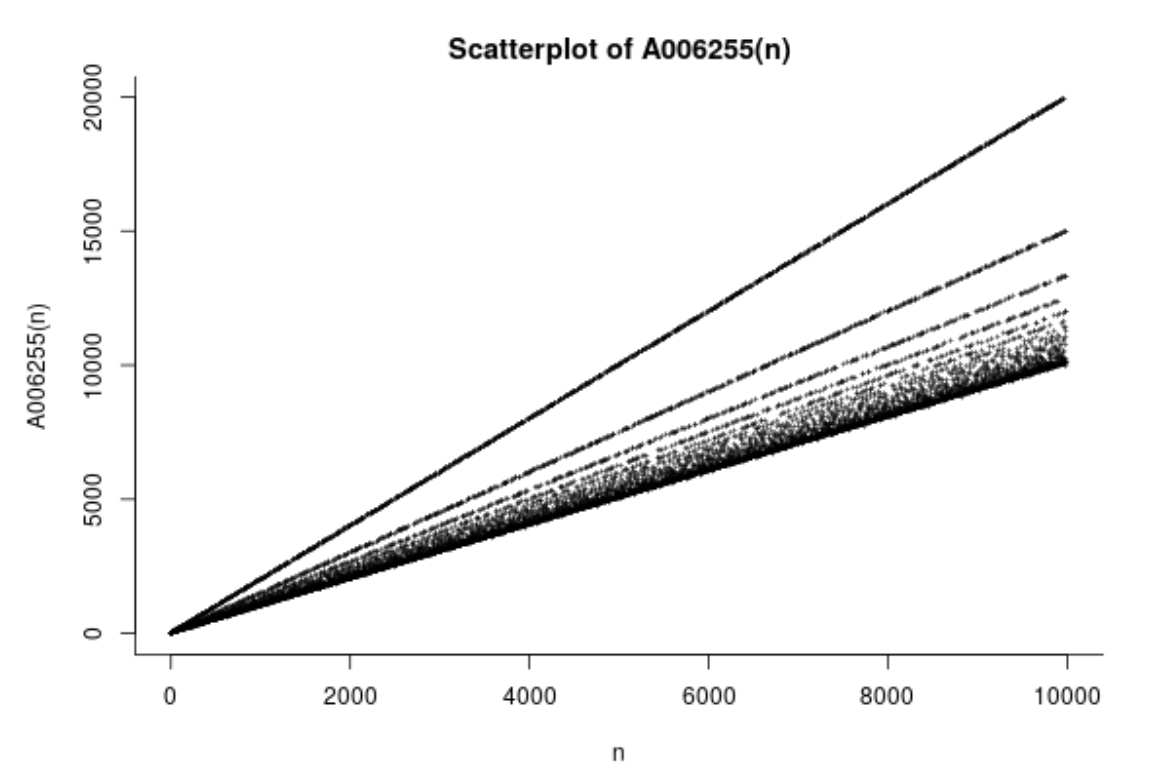
\includegraphics[width=300pt]{A006255_plot.png}}
\end{frame}

% \begin{frame}{Counting valid sequences (OEIS A259527)}
%   \begin{block}{Example}
%     42, 48, 56 \\
%     42, 48, 49, 56 \\
%     42, 50, 54, 56 \\
%     42, 49, 50, 54, 56 \\
%     42, 44, 45, 48, 55, 56 \\
%     42, 44, 45, 48, 49, 55, 56 \\
%     42, 44, 45, 50, 54, 55, 56 \\
%     42, 44, 45, 49, 50, 54, 55, 56 \\
%   \end{block}
% \end{frame}

\begin{frame}{Counting valid sequences (OEIS A259527)}

  \begin{block}{Example}
    For $n = 20$ there are four square sequences starting with $20$ and ending
    with $g(20)=30$:
    \begin{alignat*}{4}
      &20 \cdot 24 \cdot 30                                     &&= 120^2   \\
      &20 \cdot 24 \cdot 25 \cdot 30                            &&= 600^2   \\
      &20 \cdot 21 \cdot 24 \cdot 27 \cdot 28 \cdot 30          &&= 15120^2 \\
      &20 \cdot 21 \cdot 24 \cdot 25 \cdot 27 \cdot 28 \cdot 30 &&= 75600^2
    \end{alignat*}
  \end{block}
    How many square sequences in general?

\end{frame}

\begin{frame}{Counting valid sequences (OEIS A259527)}
  Once g(n) has been computed, a similar algorithm can be used to compute the
  number of sequences: \[
    n = b_1 < b_2 < \hdots < b_t = g(n)
  \]

  Again, we set up a system of equations (where $v = v_{\pi(g(n))}$): \[
    \mathcal{C}_n =
    \begin{blockarray}{ccccc}
      \begin{block}{[ccccc]}
        & & & & \\
        \vrule & \vrule   &        & \vrule      & \vrule \\
        v(n)   & v(n + 1) & \cdots & v(g(n) - 1) & v(g(n)) \\
        \vrule & \vrule   &        & \vrule      & \vrule \\
        & & & & \\
      \end{block}
    \end{blockarray}
  \]

    % Given that there is at least one valid sequence, the total number of sequences is:
    And the number of valid sequences is: \[ 2^{\operatorname{nul}(C_n) - 1} \]
\end{frame}

\begin{frame}{Counting valid sequences (Example)}

    \[
      \mathcal{C}_{20} =
      \begin{blockarray}{ccccccccccc}
    20         & 21         & & & & \cdots & & & & 29         & 30         \\
    \downarrow & \downarrow & & & &        & & & & \downarrow & \downarrow \\
      \begin{block}{[ccccccccccc]}
        0 & 0 & 1 & 0 & 1 & 0 & 1 & 0 & 0 & 0 & 1 \\
        0 & 1 & 0 & 0 & 1 & 0 & 0 & 1 & 0 & 0 & 1 \\
        1 & 0 & 0 & 0 & 0 & 0 & 0 & 0 & 0 & 0 & 1 \\
        0 & 1 & 0 & 0 & 0 & 0 & 0 & 0 & 1 & 0 & 0 \\
        0 & 0 & 1 & 0 & 0 & 0 & 0 & 0 & 0 & 0 & 0 \\
        0 & 0 & 0 & 0 & 0 & 0 & 1 & 0 & 0 & 0 & 0 \\
        0 & 0 & 0 & 0 & 0 & 0 & 0 & 0 & 0 & 0 & 0 \\
        0 & 0 & 0 & 0 & 0 & 0 & 0 & 0 & 0 & 0 & 0 \\
        0 & 0 & 0 & 1 & 0 & 0 & 0 & 0 & 0 & 0 & 0 \\
        0 & 0 & 0 & 0 & 0 & 0 & 0 & 0 & 0 & 1 & 0 \\
      \end{block}
      \end{blockarray}
    \]

\end{frame}

\begin{frame}{A basis for the null space of $\mathcal{C}_{20}$}
  \[
    \left\{
      \left[\begin{array}{c}
        1 \\ 0 \\ 0 \\ 0 \\ 1 \\ 0 \\ 0 \\ 0 \\ 0 \\ 0 \\ 1
      \end{array}\right]
      \begin{array}{cc}
        \leftarrow & 20 \\ \\ \\ \\
        \leftarrow & 24 \\ \\ \\ \\ \\ \\
        \leftarrow & 30
      \end{array},
      %----------------------------------------------------
      \left[\begin{array}{c}
        0 \\ 1 \\ 0 \\ 0 \\ 0 \\ 0 \\ 0 \\ 1 \\ 1 \\ 0 \\ 0
      \end{array}\right]
       \begin{array}{cc}
        \\ \leftarrow & 21 \\ \\ \\ \\ \\ \\
        \leftarrow & 27 \\ \leftarrow & 28 \\ \\ \\
      \end{array},
      %----------------------------------------------------
      \left[\begin{array}{c}
        0 \\ 0 \\ 0 \\ 0 \\ 0 \\ 1 \\ 0 \\ 0 \\ 0 \\ 0 \\ 0
      \end{array}\right]
      \begin{array}{cc}
        \\ \\ \\ \\ \\ \leftarrow & 25 \\ \\ \\ \\ \\ \\
      \end{array}
    \right\}
  \]

    The basis can be constructed in such a way that only one vector has $1$
    as its first and last entry.
    % Proof:
    % (1) Suppose there exists a vector with a 1 as the first entry but not as the last,
    % Then g(n) is not minimal in the construction of $\mathcal{C}_{20}$ because there is a
    % solution with a smaller upper bound.
    % (2) Suppose there exists a vector with a 1 as the last entry but not as the first,
    % Then take this vector and add it to the principal vector. We have created a new vector in the
    % null space of $\mathcal{C}_{20}$ subject to condition 1. A contradiction.
    \[
      \text{Number of square sequences: } 2^{\operatorname{nul}(C_n) - 1}
    \]
    % From the basis, we can take an arbitrary subset of ``non-solution'' vectors,
    % and add them with the ``solution'' vector to construct a new square sequence.
\end{frame}

% \begin{frame}{Counting primitive sequences (OEIS A291634)}
%   \begin{block}{Example}
%     For $n = 11$ there are eight square sequences starting with $11$ and ending
%     with $g(11)=22$, but only three such that no proper nonempty subset
%     is a square sequence:
%     \begin{alignat*}{2}
%       & \mathbf{11 \cdot 18 \cdot 22}                            &&= \mathbf{66^2} \\
%       & 11 \cdot 16 \cdot 18 \cdot 22                            &&= 264^2 \\
%       & 11 \cdot 12 \cdot 15 \cdot 18 \cdot 20 \cdot 22          &&= 3960^2 \\ % 12 \cdot 15 \cdot 20 = 60^2
%       & 11 \cdot 12 \cdot 15 \cdot 16 \cdot 18 \cdot 20 \cdot 22 &&= 15840^2 \\
%       & \mathbf{11 \cdot 12 \cdot 14 \cdot 21 \cdot 22}          &&= \mathbf{924^2} \\
%       & 11 \cdot 12 \cdot 14 \cdot 16 \cdot 21 \cdot 22          &&= 3696^2 \\
%       & \mathbf{11 \cdot 14 \cdot 15 \cdot 20 \cdot 21 \cdot 22} &&= \mathbf{4620^2} \\
%       & 11 \cdot 14 \cdot 15 \cdot 16 \cdot 20 \cdot 21 \cdot 22 &&= 18480^2 \\
%     \end{alignat*}
%     Is there a nice way to count primitive sequences?
%   \end{block}
% \end{frame}

% \begin{frame}{Generalizations}
%   Let $m$ be the smallest integer for which there exists a sequence \[
%     n = b_1 < b_2 < \cdots < b_t = m
%   \] where \begin{alignat*}{3}
%     % Note: A277278 in OEIS
%     &  \sum_{i = 1}^{t} b_i           &&= k^2         &\text{ for some } k \in \mathbb{N} \\
%     & \prod_{i = 1}^{t} b_i           &&= k^3         &\text{ for some } k \in \mathbb{N} \\
%     &  \sum_{i = 1}^{t} \frac{1}{b_i} &&= 1
%   \end{alignat*}
% \end{frame}

\begin{frame}{Generalize to cubes (OEIS A227494)}
% This talk spawned a couple new sequences.
%   (4) Generalize this to cubes.
%     (a) A277494 (Draft)

  % g(n) is defined by the least upper bound of a monotonically increasing sequence starting at n
  % with the property that the product of the sequence is a cube. In particular, we'll enforce that
  % the second term is strictly greater than n, so we can't just do n^3*(the-next-perfect-cube).
  Let $g_3(n)$ be the least $m$ for which there exists a sequence
    \[n = b_1 < b_2 \leq b_3 \leq \cdots \leq b_t = m\]
  where \[
    b_1 \cdot b_2 \cdot b_3 \cdot \hdots \cdot b_t \text{ is a cube.}
  \]
%     (b) If we loosen the constraints in a particular way, cubes should follow from doing the same as squares. But in order to have it play nice, we need to allow duplicate terms. (e.g.) $g_3(3) \leq \text{ via } 3 \cdot 4^2 \cdot 6^2 \text{ or } 3^2 \cdot 4 \cdot 6

%       (ii) The cubes problem probably has similar properties. I suspect it's also 1-to-1.
%     (c) I'm not sure if there's a trick for strict inequalities.
  % Note: This isn't strictly increasing.
    \begin{block}{Example}
    \setlength\abovedisplayskip{-10pt}
    \begin{alignat*}{3}
      & g_3(1) = 1  \quad && \rightarrow 1                                &&= 1^3 \\
      & g_3(2) = 4  \quad && \rightarrow 2 \cdot 4                        &&= 2^3 \\
      & g_3(3) = 6  \quad && \rightarrow 3 \cdot 4^2 \cdot 6^2            &&= 12^3 \\
      & g_3(4) = 9  \quad && \rightarrow 4 \cdot 6   \cdot 9              &&= 6^3 \\
      & g_3(5) = 10 \quad && \rightarrow 5 \cdot 6   \cdot 9   \cdot 10^2 &&= 30^3
    \end{alignat*}
    \end{block}
\end{frame}

\begin{frame}{Generalize to cubes (OEIS A227494)}

  % Build up the matrix
    \[
    \mathcal{M}_{3, 3} = % Haha! You can't tell which 3 is which!
    % I've chosen to have columns up to 6 because I know the solution, but we need `
    % `sufficiently many'' columns here
    \begin{blockarray}{ccccc}
        4          & 5           & 6           & 3          \\
          \downarrow & \downarrow  & \downarrow  & \downarrow \\
    \begin{block}{[ccc|c]c}
%       4   5   6   3
        2 & 0 & 1 & 0 & \leftarrow 2 \\
        0 & 0 & 1 & 1 & \leftarrow 3 \\
        0 & 1 & 0 & 0 & \leftarrow 5 \\
    \end{block}
    \end{blockarray}
    \]

  % RREF
    \[
    \text{rref}(\mathcal{M}_{3, 3}) =
    % This is also bounded above by 2n, which can be proven with the same argument I can prove
    % analytically that the bound holds for n > 117, and a case by case basis for all n > 4.
    % The same lower bound explored earlier (for the original version of the sequence) also holds.
    \begin{blockarray}{cccc}
    \begin{block}{[ccc|c]}
%       4   5   6   3
        1 & 0 & 0 & 1 \\
        0 & 1 & 0 & 0 \\
        0 & 0 & 1 & 1 \\
    \end{block}
    \end{blockarray}
    \]

    % We're going to multiply this by the multiplicative inverse if necessary.
    Thus $g_3(3) = 6$ via $3 \cdot 4^2 \cdot 6^2$ given by the solution \[
      \begin{blockarray}{cccc}
      \begin{block}{[cccc]}
      2 & 0 & 2 & 1 \\
      \end{block}
      \end{blockarray}^T
    \]

    % Can we generalize this any further? Sure, for primes. But composite powers lack the field
    % properties needed to do this. Perhaps we could be inventive with linear algebra over a
    % Commutative ring with identity, but that's above my pay grade.
\end{frame}
% Composite powers
% LCM
% counting primitive sequences
\begin{frame}{Generalizations}
  \begin{itemize}
    \item Powers greater than 3.
      \begin{itemize}
        \item Powers that are prime follow a similar construction.
        \item The above construction does not work for composite powers.
      \end{itemize}
    \item Counting number of subsequences of a finite sequence with a square
      product.
    \item Sequences such that the $\operatorname{LCM}$ is square (OEIS A300516).
    \item Sequences such that no proper nonempty subsequence has a
      square product.
  \end{itemize}
	% \begin{block}{}
	% $\mathbb{Z}_4$ is not a field.\\
	% Assign numbers to the elements of $\mathbb{F}_4$, and find powers of 4 under a funny operation.
  % \end{block}
	% \begin{block}{Prime powers}
  %   Generalize similarly to the cube sequence.
  % \end{block}
  % \begin{block}{Nonconsecutive sequences}
  % The algorithm can find and count square subsets (or cube subsets, etc) of arbitrary sets of integers.
  % \end{block}
\end{frame}
% \begin{frame}{Does the technique generalize?}
%     \begin{itemize}
%       \item Generalizes nicely to prime powers
%         \item Breaks down for composite powers because of missing field properties
%           % particularly multiplicative inverses
%       % \item Linear algebra over a commutative ring with identity.
%           % Which seems cool, but I don't know how real that is.
%       % In any case, it looks out of my pay grade.
%             % If this is a thing, and it's cool, chat with me afterward.
%   \end{itemize}
% \end{frame}

% \begin{frame}{Generalize to sums (A277278)}
%     % You can do it (and I did!)
%     % But (unsurprisingly) there don't seem to be any obviously nice properties.
%
%   Let $g_+(n)$ be the smallest $m$ for which there exists a sequence
%     \[n = b_1 < b_2 < \cdots < b_t = m\]
%   where
%     \[\sum_{i = 1}^{t} b_i = k^2 \text{ for some } k \in \mathbb{N}\]
%
%   \begin{block}{Examples}
%     \setlength\abovedisplayskip{-10pt}
%     \begin{alignat*}{3}
%       & g_+(2) = 4  && \qquad\quad 2 + 3 + 4          &&= 3^2 \\
%       & g_+(3) = 6  && \qquad\quad 3 + 6              &&= 3^2 \\
%       & g_+(4) = 4  && \qquad\quad 4                  &&= 2^2 \\
%       & g_+(5) = 10 && \qquad\quad 5 + 6 + 7 + 8 + 10 &&= 6^2
%     \end{alignat*}
%
%     0, 1, 4, 6, 4, 10, 10, 9, 14, 9, 14, 13, 13, 18, 18, 18, 16, 19, 22, 23, 23, 27, 27, 26, 25, 25, 28, 33, 32, 35, 34, 33, 35, 38, 38, 40, 36, 42, 42, 42, 41, 48, 48, 47, 51, 50, 50, 49, 52, 49, 57, 57, 59, 59, 58, 58, 63, 63, 63, 62, 61, 66, 66, 67, 64, 73, 73, ...
%     \end{block}
% \end{frame}

% \begin{frame}{Generalize to LCM (OEIS A300516)}
%     % You can do it (and I did!)
%     % Bounded above by the the least square multiple of square of the
%     % squarefree part that is larger than n.
%
%   Let $g_{LCM}(n)$ be the smallest $m$ for which there exists a sequence
%     \[n = b_1 < b_2 < \cdots < b_t = m\]
%   where
%     \[
%       \text{LCM}/(a_1, a_2, ... a_t) =
%       k^2 \text{ for some } k \in \mathbb{N}
%      \]
%
%   \begin{block}{Examples}
%     \setlength\abovedisplayskip{-10pt}
%     \begin{alignat*}{3}
%       & g_{LCM}(6)  = 12 && \qquad\quad LCM/(6, 9, 12)   &&= 6^2 \\
%       & g_{LCM}(7)  = 49 && \qquad\quad LCM(7, 49)       &&= 7^2 \\
%       & g_{LCM}(8)  = 16 && \qquad\quad LCM(8, 16)       &&= 4^2 \\
%         % Because 1 is the identity on LCM
%         & g_{LCM}(9)  = 9  && \qquad\quad LCM(1, 9)        &&= 3^2 \\
%         & g_{LCM}(10) = 25 && \qquad\quad LCM/(10, 16, 25) &&= 20^2 \\
%         & g_{LCM}(20) = 25 && \qquad\quad LCM(20, 25)      &&= 10^2
%     \end{alignat*}
%   \end{block}
% \end{frame}

% \begin{frame}{Optimization}
%     % Going back to the original sequence (square product)
%   \[
%      \text{Let } S_n =
%       \left\{ \{b_i\}_{i=1}^t \text{ a square sequence} \mid\
%           b_1 = n,
%             b_t = g(n)
%       \right\}
%     \]
%      % Let S_n be the set of sequences starting with n and ending with g(n) whose product is a perfect square
%
%     % We could, of course, do the same thing for maximization,
%     % maybe we want the maximum GCD or something.
%
%     Find the "best" sequences in $S_n$: \\
%     \begin{itemize}
%       % I'm sure there's a good linear algebra technique that will illuminate some of these
%       % Especially number of terms. Maybe minimum product?
%       \item Number of primitive sequences
%       \item Minimum product %$\min\{\prod_{s \in S} s | S \in S_n\}$
%       \item Maximum product %$\min\{\prod_{s \in S} s | S \in S_n\}$
%       \item Minimum sum
%       \item Minimum number of distinct prime factors
%       \item Minimum number of terms (A066400)
%       \item Maximum number of terms
%       \item Minimum LCM
%       \item Maximum GCD
%      \end{itemize}
% \end{frame}

\begin{frame}{Final Conjecture}
  \begin{block}{Conjecture (Robert G. Wilson v, 2002)}
    \[n\cdot g(n) \text{ is nonsquare for all nonsquare } n \in \mathbb{N}\]
  \end{block}
  \center{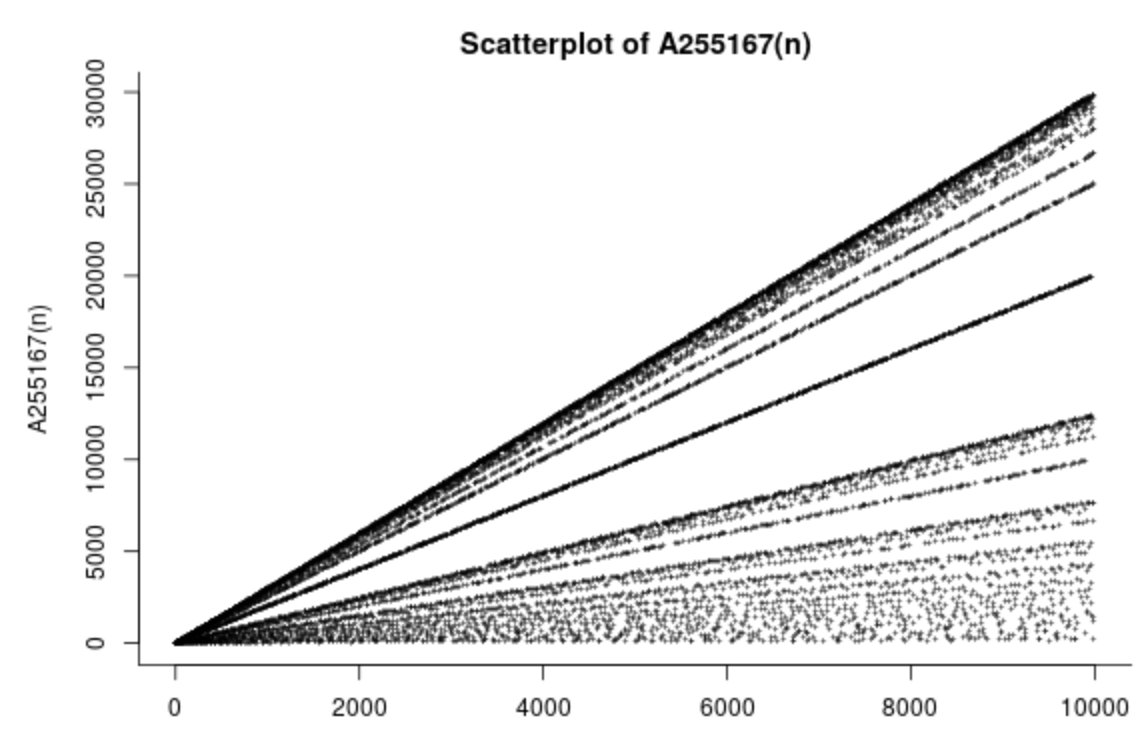
\includegraphics[width=240pt]{A255167_plot.png}}
\end{frame}

\end{document}
